\documentclass{beamer}
\usepackage{etex}
\reserveinserts{28}
\usepackage[utf8]{inputenc}
\usepackage[T1]{fontenc}
\usepackage{xspace}
% \usepackage[colorlinks=true]{hyperref}
\usepackage{color}

\usepackage{amsmath}
\usepackage{amssymb,amsthm,amsfonts}


\newtheorem{thm}{Theorem}
\newtheorem{cor}[thm]{Corollary}
\newtheorem{prop}[thm]{Proposition}
\newtheorem{defi}[thm]{Definition}
\newtheorem{lem}[thm]{Lemma}
\newtheorem{ax}[thm]{Axiom}

\newcommand \defeq {\overset{de\hspace{-0.2ex}f}{=}}

\newcommand{\mynote}[2]{
  \fbox{\bfseries\sffamily\scriptsize#1}
  {\small$\blacktriangleright$\textsf{\emph{#2}}$\blacktriangleleft$}~}

\newcommand\kq[1]{\mynote{KQ}{#1}}
\newcommand\nt[1]{\mynote{NT}{#1}}

\newcommand{\ie}{i.e,\xspace}
\newcommand{\eg}{e.g,\xspace}

% correct bad hyphenation here
\hyphenation{op-tical net-works semi-conduc-tor}


\usepackage{enumerate}
\usepackage{wasysym}

\mode<beamer>{%
  \usetheme[right,width=22mm]{Goettingen}
}

\AtBeginSection[]{
  \begin{frame}<beamer>{}
    \tableofcontents[currentsection,currentsubsection]
    \note{ }
  \end{frame}
}

\setbeamertemplate{navigation symbols}{} 
\usepackage{pgfpages}
\setbeameroption{show notes on second screen=right}

\usepackage{bussproofs}


\usepackage[all]{xy}
\def\dar[#1]#2{\ar@<-#2>[#1]\ar@<#2>[#1]} %double arrows in xy
\def\tar[#1]#2{\ar@<#2>[#1]\ar@<0pt>[#1]\ar@<-#2>[#1]} %triple arrows in xy
\DeclareMathOperator{\Type}{Type}
\DeclareMathOperator{\HProp}{HProp}
\DeclareMathOperator{\HSet}{HSet}
\DeclareMathOperator{\IsHProp}{IsHProp}
\DeclareMathOperator{\IsHSet}{IsHSet}
\DeclareMathOperator{\nat}{nat}
\DeclareMathOperator{\Unit}{Unit}
\DeclareMathOperator{\im}{Im}
\DeclareMathOperator{\id}{id}
\DeclareMathOperator{\Contr}{Contr}
\DeclareMathOperator{\IsContr}{IsContr}
\DeclareMathOperator{\IsEquiv}{IsEquiv}
\DeclareMathOperator{\precompose}{\mathrm{precompose}}
\DeclareMathOperator{\postcompose}{\mathrm{postcompose}}
\DeclareMathOperator{\idmap}{\mathrm{idmap}}
\DeclareMathOperator{\cocone}{cocone}
\DeclareMathOperator{\inl}{inl}
\DeclareMathOperator{\inr}{inr}
\DeclareMathOperator{\transport}{transport}
\DeclareMathOperator{\tr}{tr}
\DeclareMathOperator{\Sym}{Sym}
\DeclareMathOperator{\Trans}{Trans}
\DeclareMathOperator{\Refl}{Refl}


\def\mymathhyphen{{\hbox{-}}}

\newcommand{\IsType}[1]
{\mathop{\mathrm{Is\mymathhyphen}#1\mathrm{\mymathhyphen type}} }

\newcommand{\modal}{\ensuremath{\ocircle}}
\newcommand \True {\top}
\newcommand \idpath {\mathrm{idpath}}
\newcommand \False {\bot}
\newcommand \closure[1] {\overline{#1}}
\newcommand \Char[1] {\chi_{#1}}%{\mathrm{char}(#1)}
\newcommand \E {\mathcal{E}}
\newcommand \Hom[1] {\mathrm{Hom}_{#1}}
\newcommand \Obj {\mathrm{Obj}}
\newcommand \Sh[1] {\mathrm{Sh}_{#1}}
\newcommand \squash[1] {\| #1 \| }
\newcommand \separated {\mathop{\square_{n+1}} }
\newcommand \fib[2] {\mathrm{fib}_{#1}(#2)}
\newcommand \colim {\mathrm{colim}}
\newcommand \zero {\mathbf{0}}
\newcommand \one {\mathbf{1}}
\newcommand \unittt{\star}
\newcommand \two {\mathbf{2}}
\newcommand{\sumD}[3]{\sum_{#1:#2}\, #3}
\newcommand{\prodD}[3]{\prod_{#1:#2}\, #3}
\newcommand{\homot}{\sim}
\newcommand{\retr}{\mathrm{retr}}
\newcommand{\sect}{\mathrm{sect}}
\newcommand{\adj}{\mathrm{adj}}
\newcommand{\ap}[1]{\mathrm{ap}_{#1}}
\newcommand{\inv}[1]{#1^{-1}}
\newcommand{\concat}[2]{#1\cdot #2}
\newcommand{\happly}{\mathrm{happly}}
\newcommand{\Sone}{\mathbb{S}^1}
\newcommand{\baseS}{\mathrm{base}}
\newcommand{\loopS}{\mathrm{loop}}
\newcommand{\coeq}[2]{\mathrm{Coeq}^{#1,#2}}

\DeclareMathOperator{\issep}{IsSeparated}
\DeclareMathOperator{\issheaf}{IsSheaf}
\DeclareMathOperator{\KP}{KP}
\DeclareMathOperator{\kp}{kp}

\title{Lawvere-Tierney Sheafification\\ in Homotopy Type Theory}

\author{{Kevin Quirin} \\ 
  {Mines de Nantes \\ Nantes, France}}

\date{29 June 2015}

\begin{document}

\begin{frame}
    
    \note{Thank you all for coming, especially the members of the
      committee. It is a great honour for me to have such a great
      comittee for my defence.

    I will present you my work on sheafification in homotopy type theory}
    \maketitle
    
\end{frame}

\section[Type Theory]{Introduction to type theory}
\label{sec:intr-type-theory}

\begin{frame}
  \frametitle{Foo}
  Bar
\end{frame}

\subsection[Proof]{Formalizing proofs}
\label{sec:formalizing-proofs}

\begin{frame}
  \frametitle{Errors in mathematics}
  
  One issue with mathematics: it is hard to check proofs.
  \begin{center}
    

  % \begin{center}
    \frame{
      \includegraphics<2,3>[scale=0.3]{spencer_bloch}}
    \note[item]{In a paper by Spencer Bloch, Suslin found an error in lemma
      1.1. Almost all the paper ws relying on this lemma}
  % \end{center}
  \llap{%
    % \begin{center}
    \frame{\includegraphics<3>[scale=0.35]{bloch_lemma}}
    % \end{center}
  }
  \end{center}
  \note<2->[item]{While the original - false - proof was only a few lines long,
    the new proof is about thirty pages long, and contains complex arguments.}
  \onslide<4>{
    Proofs are more and more complicated.
  }

\end{frame}

\begin{frame}[c]
  \centering


  \note<1->[item]{If you give a proof to the best mathematician}
  \note<2->[item]{He will probably don't know if it is true or not}
  \note<3->[item]{Our hope is to give to rather to a computer}
  \note<4->[item]{Who can decide if it is right or wrong, and in the
    latter case, where is the error}
  \begin{tabular}{ccc}
  % \begin{center}
    \onslide<1,3>{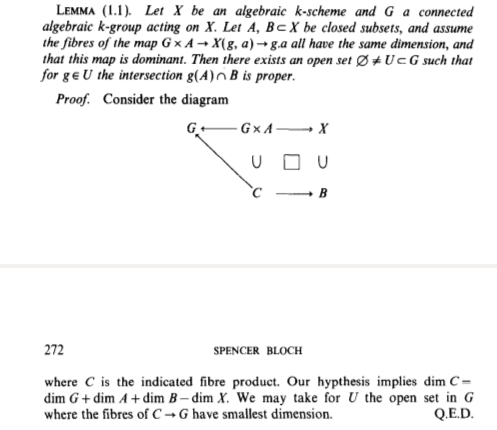
\includegraphics[scale=0.15]{bloch_lemma}} &
    \only<1,2>{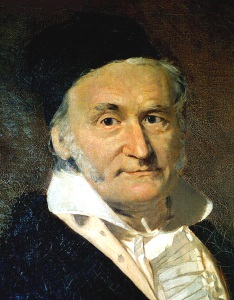
\includegraphics[scale=0.7]{gauss}}
    \only<3,4>{
\includegraphics[scale=0.25]{computer}
      
}
      &
      \begin{overprint}
        \onslide<2>{\quad\Large Ich wei\ss{} nicht }
        \onslide<4>{\hspace{-8em}\begin{tabular}[x]{@{}c@{}}False\\Error
            on line 4\end{tabular}}
      \end{overprint}

    
  % \end{center}
  \end{tabular}
\end{frame}

\subsection[Curry-Howard]{The Curry-Howard isomorphism}
\label{sec:curry-howard-isom}

\begin{frame}
  \frametitle{Curry-Howard}
  
  As the previous section suggests, it is a good idea to know what is
  a correct proof.

  \vspace{2em}
  This part of mathematics is called {\em proof theory}.

  \vspace{2em}
  It describes how to be sure that a proof is correct.
\end{frame}

\begin{frame}

  \begin{center}
    \AxiomC{}
    \UnaryInfC{$\Gamma\vdash \top$}
    \DisplayProof
    \qquad
    \AxiomC{$\Gamma,A\vdash B$}
    \UnaryInfC{$\Gamma \vdash A \Rightarrow B$}
    \DisplayProof
  \end{center}
\begin{center}
    \AxiomC{$\Gamma \vdash A$}
    \AxiomC{$\Gamma \vdash B$}
    \BinaryInfC{$\Gamma \vdash A\land B$}
    \DisplayProof
  \end{center}
  \begin{center}
    \AxiomC{$\Gamma\vdash A$}
    \UnaryInfC{$\Gamma\vdash A\lor B$}
    \DisplayProof
    \qquad
    \AxiomC{$\Gamma \vdash B$}
    \UnaryInfC{$\Gamma\vdash A\lor B$}
    \DisplayProof
  \end{center}
\end{frame}

\begin{frame}
  These rules really look like the ones of lambda-calculus, the most
  simple programming language~: 

    \begin{center}
    \AxiomC{}
    \UnaryInfC{$\Gamma\vdash \onslide<2>{\unittt\,:\,} \top$}
    \DisplayProof
    \qquad
    \AxiomC{$\Gamma,\onslide<2>{a\,:\,}A\vdash \onslide<2>{b\,:\,}B$}
    \UnaryInfC{$\Gamma \vdash A \Rightarrow B$}
    \DisplayProof
 \end{center}
\begin{center}
    \AxiomC{$\Gamma \vdash \onslide<2>{a\,:\,}A$}
    \AxiomC{$\Gamma \vdash  \onslide<2>{b\,:\,}B$}
    \BinaryInfC{$\Gamma \vdash \onslide<2>{(a,b)\,:\,} A\land B$}
    \DisplayProof
  \end{center}
  \begin{center}
    \AxiomC{$\Gamma\vdash \onslide<2>{a\,:\,}A$}
    \UnaryInfC{$\Gamma\vdash \onslide<2>{\inl a\,:\,}A\lor B$}
    \DisplayProof
    \qquad
    \AxiomC{$\Gamma \vdash \onslide<2>{b\,:\,} B$}
    \UnaryInfC{$\Gamma\vdash \onslide<2>{\inr b\,:\,}A\lor B$}
    \DisplayProof
  \end{center}
\end{frame}

\begin{frame}
  The Curry-Howard isomorphism states that if a term of a type can be
  seen as a program, it can also be seen as a proof of a formula.
\end{frame}

\section[Forcing]{Forcing and Sheafification}
\label{sec:forc-sheaf}

\section[Sheafification]{Lawvere-Tierney Sheafification in Type Theory}
\label{sec:sheaf-type-theory}





\end{document}
